\iffalse
\documentclass[12pt]{article}
\usepackage{graphicx}
\usepackage{amsmath}
\usepackage{mathtools}
\usepackage{gensymb}

\newcommand{\mydet}[1]{\ensuremath{\begin{vmatrix}#1\end{vmatrix}}}
\providecommand{\brak}[1]{\ensuremath{\left(#1\right)}}
\providecommand{\norm}[1]{\left\lVert#1\right\rVert}
\newcommand{\solution}{\noindent \textbf{Solution: }}
\newcommand{\myvec}[1]{\ensuremath{\begin{pmatrix}#1\end{pmatrix}}}
\let\vec\mathbf

\begin{document}
\begin{center}
\textbf\large{CHAPTER-7 \\ COORDINATE GEOMETRY}
\end{center}
\section*{Excercise 7.2}

1. Find the coordinates of the point which divides the join $\vec(-1,7) \text{ and } \vec(4,-3)$ in the ratio 2:3 :
\\
\\
\solution\\		
\fi
The coordinates and ratio are given as
\begin{align}
\vec{P}=\myvec{-1\\7\\},
\vec{Q}=\myvec{4\\-3\\},
n=\frac{3}{2}
\end{align}
Using section formula
\begin{align}
\vec{R}&=\frac{\vec{Q}+n\vec{P}}{1+n}\\
&=\frac{1}{1+\frac{3}{2}}  \myvec{\myvec{
4\\
-3\\
}
  +
   \frac{3}{2}\myvec{
-1\\
7\\
}}\\
&=\myvec{
1\\
3
}
\end{align}
See Fig. 
\ref{fig:chapters/10/7/2/1/Fig}
\begin{figure}[!h]
\begin{center}
   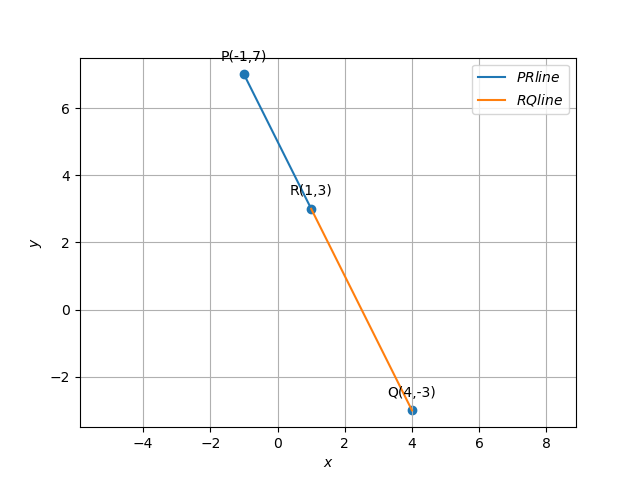
\includegraphics[width=\columnwidth]{chapters/10/7/2/1/figs/linefig.png}
\end{center}
\caption{}
\label{fig:chapters/10/7/2/1/Fig}
\end{figure}

